\section{Emblemetrics}
\label{app:emblemetrics}

\begin{figure}[ht]
  \centering
  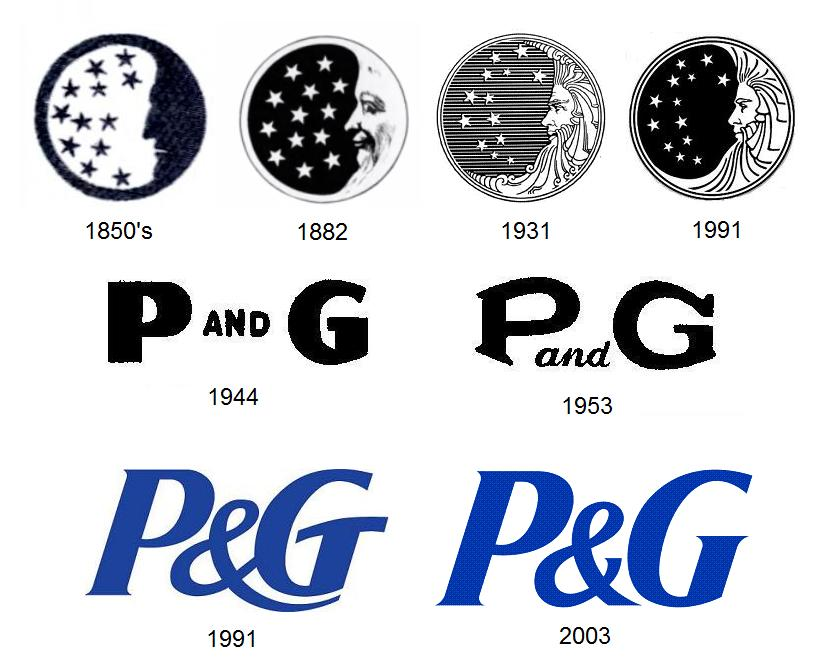
\includegraphics[width=.5\linewidth]{images/supplement/emblemetrics/pg2003}
  \caption[]{Логотипы P\&G до 2003}
  \label{fig:emblemetrics:pg2003}
\end{figure}

\begin{figure}[ht]
  \centering
  
\includegraphics[width=.3\linewidth]{images/supplement/emblemetrics/pg2013}
  \caption[]{Обновлённый логотип P\&G 2013}
  \label{fig:emblemetrics:pg2013}
\end{figure}

\begin{figure}[ht]
  \centering
  
\includegraphics[width=.5\linewidth]{images/supplement/emblemetrics/frankenmarks}
  \caption[]{Frankenmarks}
  \label{fig:emblemetrics:frankenmarks}
\end{figure}

\begin{figure}[ht]
  \centering
  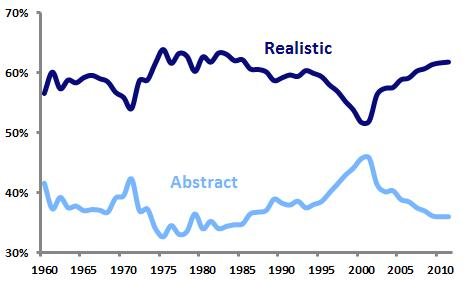
\includegraphics[width=.5\linewidth]{images/supplement/emblemetrics/abstractrealistic}
  \caption[]{Abstract and realistic logos as a percentage of all new US logos}
  \label{fig:emblemetrics:abstract-realistic}
\end{figure}

\begin{figure}[ht]
  \centering
  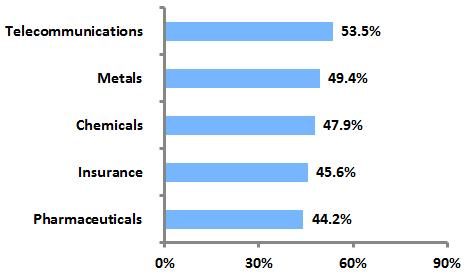
\includegraphics[width=.5\linewidth]{images/supplement/emblemetrics/highabstract}
  \caption[]{Industries with high rates of abstract logo use}
  \label{fig:emblemetrics:high-abstract}
\end{figure}

\begin{figure}[ht]
  \centering
  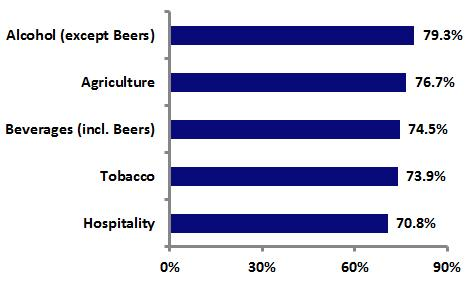
\includegraphics[width=.5\linewidth]{images/supplement/emblemetrics/highrealistic}
  \caption[]{Industries with high rates of realistic logo use}
  \label{fig:emblemetrics:high-realistic}
\end{figure}

\begin{figure}[ht]
  \centering
  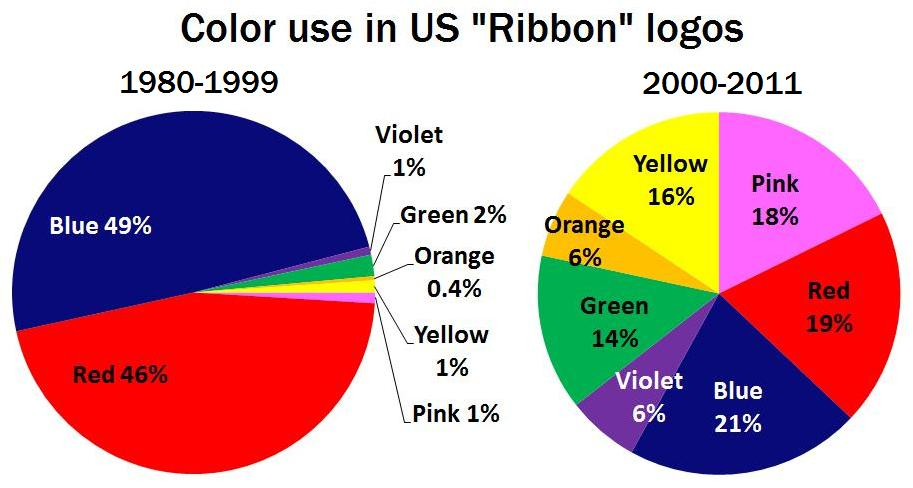
\includegraphics[width=.5\linewidth]{images/supplement/emblemetrics/coloruse}
  \caption[]{Color use in US Ribbon logos}
  \label{fig:emblemetrics:color-use}
\end{figure}

\begin{figure}[ht]
  \centering
  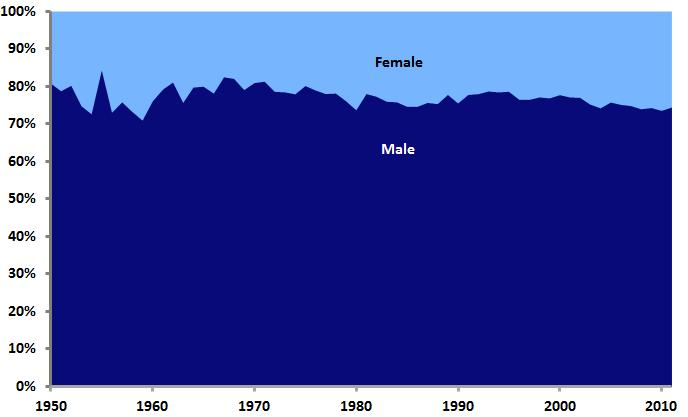
\includegraphics[width=.5\linewidth]{images/supplement/emblemetrics/malefemale}
  \caption[]{Percentage of new <<gendered>> logos featuring male or female design elements}
  \label{fig:emblemetrics:male-female}
\end{figure}

\begin{figure}[ht]
  \centering
  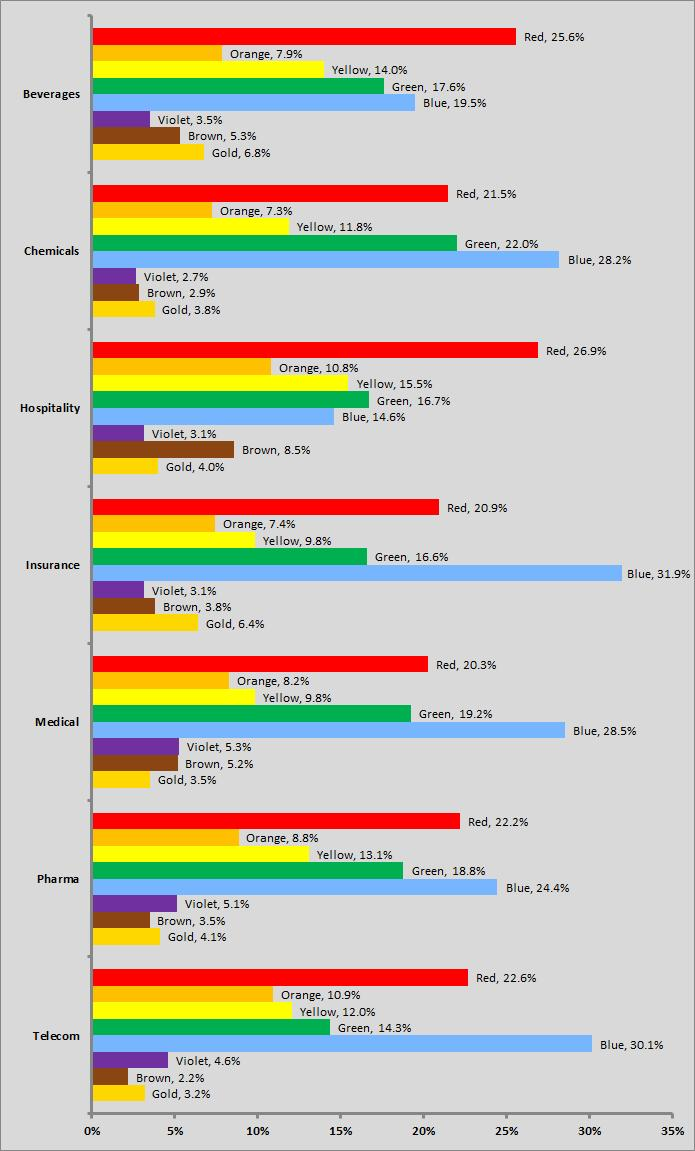
\includegraphics[width=.5\linewidth]{images/supplement/emblemetrics/colorindustry}
  \caption[]{Use of Color in US Logos by Industry}
  \label{fig:emblemetrics:color-industry}
\end{figure}

\begin{figure}[ht]
  \centering
  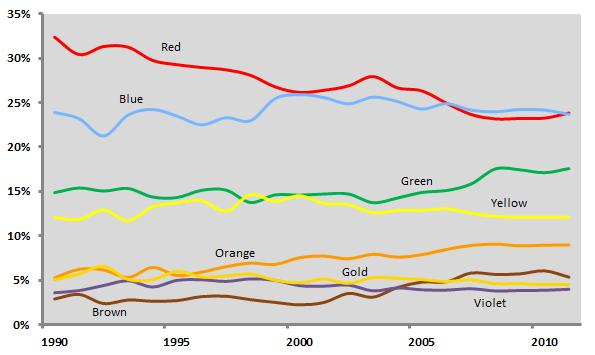
\includegraphics[width=.5\linewidth]{images/supplement/emblemetrics/color}
  \caption[]{Use of Color in US Logos}
  \label{fig:emblemetrics:color}
\end{figure}

\begin{figure}[ht]
  \centering
  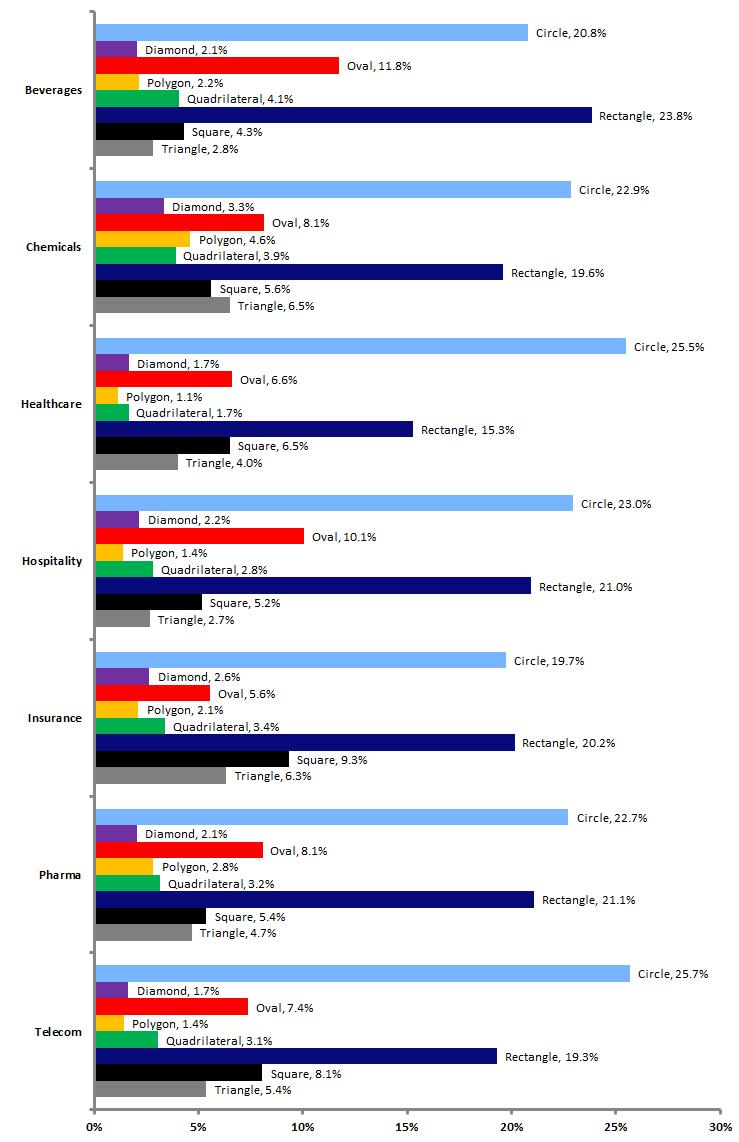
\includegraphics[width=.5\linewidth]{images/supplement/emblemetrics/shapeindustry}
  \caption[]{Percentage of logos featuring shape elements by industry}
  \label{fig:emblemetrics:shape-industry}
\end{figure}

\begin{figure}[ht]
  \centering
  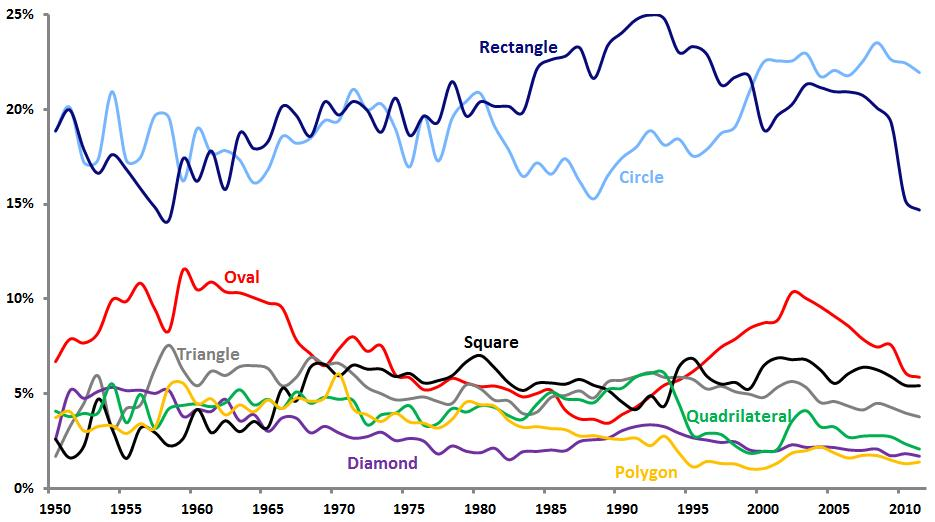
\includegraphics[width=.5\linewidth]{images/supplement/emblemetrics/shape}
  \caption[]{Percentage of new logos featuring specific shape elements}
  \label{fig:emblemetrics:shape}
\end{figure}

\begin{figure}[ht]
  \centering
  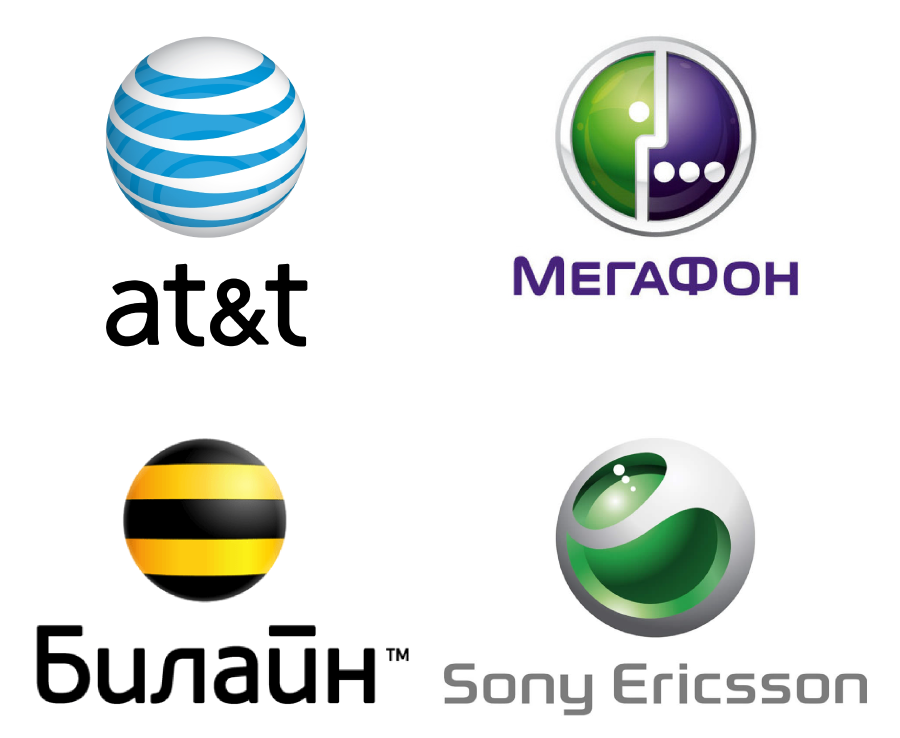
\includegraphics[width=.5\linewidth]{images/supplement/emblemetrics/web20}
  \caption[]{Логотипы операторов сотовой связи, выполненные в стилистике веб 2.0}
  \label{fig:emblemetrics:web20}
\end{figure}
